\documentclass[letterpaper]{article}
\usepackage{graphicx} 	% For figures and images
\usepackage{alltt} 		% For better verbatim

% \usepackage{fullpage}

% The HRule command is required for the title page
% from the wikibook
\newcommand{\HRule}{\rule{\linewidth}{0.5mm}}

% Change the paragraphs to block style
\setlength{\parindent}{0pt}
\setlength{\parskip}{2ex}

\begin{document}

\section{The Sailcode Application Interface} % (fold)
\label{sec:The Sailcode Application Interface}

The goal of this software rewrite is to make the code more modular. Modular code can be changed without worrying about breaking other parts of the code. Whenever a change is made to a module, we will run a \emph{unit test} to check to make sure that it performs the same operation by handling the same input and output. This way if something has been changed in such a way that it would break other parts of the code, we will know.

The new API is going to contain as much code which has already been written in an effort to save time, since a lot of work went into it which did produce some good results.

\begin{figure}[h]
	\centering
	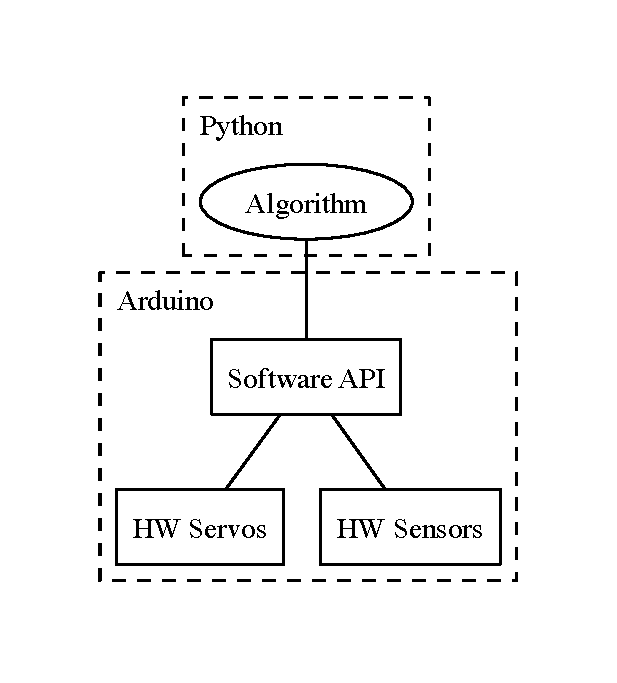
\includegraphics[width=0.8\linewidth]{mindmap_test/overview.pdf}
	\caption{Rough overview of software location}
	\label{fig:overview}
\end{figure}

% section The Sailcode Application Interface (end)

\section{Classes in Arduino} % (fold)
\label{sec:Classes in Arduino}

Although Arduino is written in C, it is possible to create classes with some limitations. You can create a Library in a seperate file/folder, which is compiled separately. Then in the Arduino source code, you can just include it and create an instance.

You cannot use the \verb:new: keyword in C, but if you really need to declare an object off the heap, you can use the relloc and malloc functions which can do the same thing. Though these would be pretty dangerous if there ever to be a memory leak.

% section Classes in Arduino (end)

\section{The Wind Sensor} % (fold)
\label{sec:The Wind Sensor}

Will be contained in its own class and carry all of its own supporting variables.

The sensor will just keep sending serial data at intervals rather than waiting for a command, so we have to have a way to keep the most recent value stored. This could mean having it update every-single time it gets a new string, then have the values ready for when a function is called, or it could ignore all messages until a function is called which requests an update of the variables.

\begin{figure}[h]
	\centering
	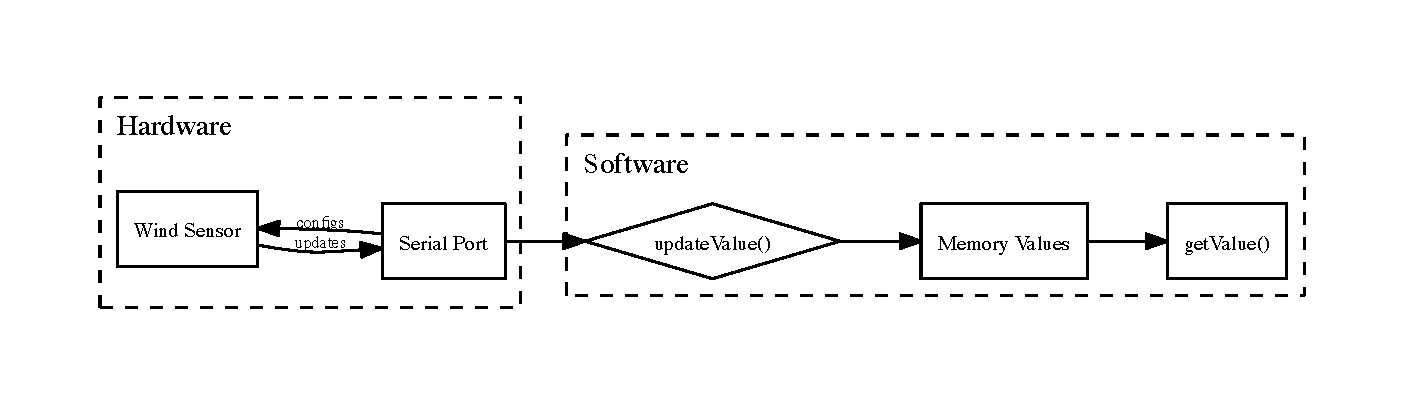
\includegraphics[width=\linewidth]{maps/WindSerial.pdf}
	\caption{Wind Sensor to Memory path}
	\label{fig:WindSensorMap}
\end{figure}



% section The Wind Sensor (end)

\end{document}
